\documentclass[aspectratio=169,11pt]{beamer}

\usepackage[utf8]{inputenc}
\usepackage[T1]{fontenc}
\usepackage[spanish,es-nodecimaldot]{babel}
\usepackage{lmodern}
\usepackage{booktabs}
\usepackage{array}
\usepackage{ragged2e}
\usepackage{xcolor}

\definecolor{Navy}{HTML}{17243A}
\definecolor{Teal}{HTML}{087E83}
\definecolor{Coral}{HTML}{E56B52}
\definecolor{Gold}{HTML}{E6A23C}
\definecolor{Pale}{HTML}{F2F5F8}
\definecolor{Muted}{HTML}{607080}
\definecolor{Green}{HTML}{32866E}


\setbeamertemplate{frametitle}{%
  \vspace{.35em}\insertframetitle\par\vspace{.15em}%
  {\color{Teal}\rule{.12\paperwidth}{2pt}}\vspace{.2em}
}
\setlength{\leftmargini}{1.4em}
\setlength{\leftmarginii}{1.2em}

\newcommand{\tagline}[1]{{\color{Teal}\bfseries\small #1}}
\newcommand{\smallnote}[1]{{\color{Muted}\scriptsize #1}}
\newcommand{\strong}[1]{{\color{Navy}\bfseries #1}}
\newcommand{\evidence}[1]{\par\vspace{.25em}{\color{Muted}\scriptsize Evidencia revisada: #1}}

\title{Limitaciones de Five Nights of Terror}
\subtitle{Análisis desde las interfaces 3D y la accesibilidad en HCI}
\author{Proyecto de Interacción Humano--Computador}
\institute{Análisis del prototipo Unity + Flutter}
\date{}

\begin{document}

% 1
\begin{frame}[plain]
  \setbeamercolor{titlelike}{fg=white,bg=Navy}
  \begin{beamercolorbox}[wd=\paperwidth,ht=\paperheight,sep=1.2cm,center]{titlelike}
    {\LARGE\bfseries Limitaciones de Five Nights of Terror}\par\vspace{.55cm}
    {\large Marcelo Torres y Anthony Briceño}\par\vspace{1cm}
  \end{beamercolorbox}
\end{frame}

% 2
\begin{frame}{El reto central del proyecto}
  \begin{columns}[T,onlytextwidth]
    \column{.55\textwidth}
      \tagline{Una experiencia repartida entre dos dispositivos}
      \vspace{.35em}
      \begin{itemize}
        \item En el \strong{PC}, el jugador vigila la escena 3D y a los animatrónicos.
        \item En la \strong{tablet}, elige tareas, resuelve minijuegos y atiende la caja musical.
        \item La cámara estima si la persona está mirando al PC.
      \end{itemize}
      \vspace{.15em}
      \begin{block}{Pregunta de evaluación}
        ¿Puede el jugador percibir, comprender y ejecutar las acciones necesarias sin que la cámara, el tiempo o el cambio de pantalla le impongan una barrera?
      \end{block}
    \column{.4\textwidth}
      \centering
      \vspace{.35cm}
      \fcolorbox{Teal}{Pale}{\parbox{.86\linewidth}{\centering\textbf{PC / Unity}\\ escena 3D + vigilancia\\[.4em]\Large $\updownarrow$\\[.4em]\textbf{Tablet / Flutter}\\ menú + minijuegos}}
      \vspace{.4cm}
      \smallnote{La atención cambia de un dispositivo al otro mientras la partida continúa.}
  \end{columns}
\end{frame}

%3

\begin{frame}{Capturas del prototipo en la tablet}
  \begin{columns}[T,onlytextwidth]

    \begin{column}{0.48\textwidth}
      \centering
      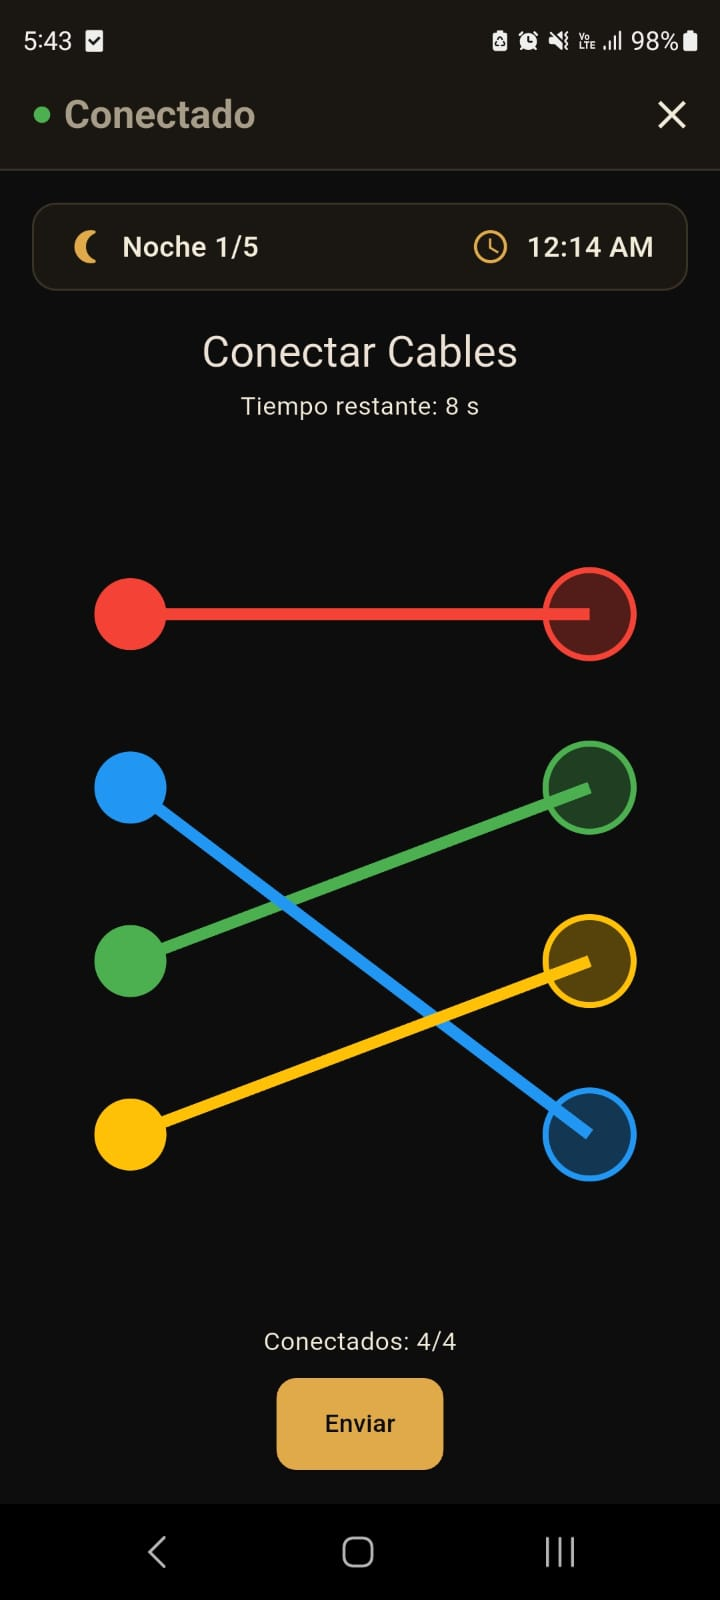
\includegraphics[
        width=\linewidth,
        height=0.62\textheight,
        keepaspectratio
      ]{imagen-1.jpeg}

      \small Minijuego rítmico
    \end{column}

    \begin{column}{0.48\textwidth}
      \centering
      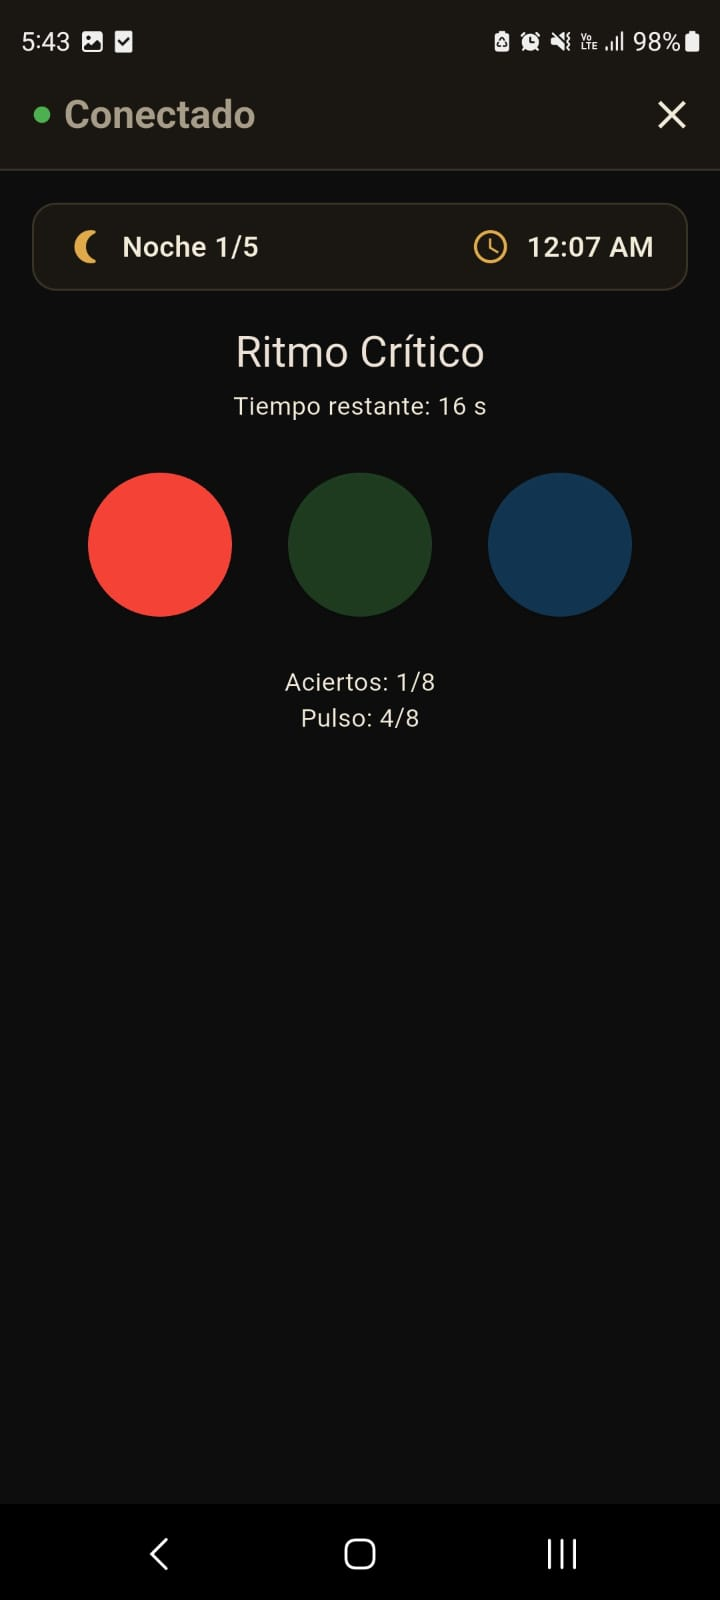
\includegraphics[
        width=\linewidth,
        height=0.62\textheight,
        keepaspectratio
      ]{imagen-2.jpeg}

      \small Minijuego de conectar cables
    \end{column}

  \end{columns}
\end{frame}
% 4
\begin{frame}{Dos marcos para analizar las limitaciones}
  \begin{columns}[T,onlytextwidth]
    \column{.48\textwidth}
      \begin{block}{Paper New Directions: diseñar la interacción 3D}
        \begin{itemize}
          \item \strong{Especificidad:} adaptar a tarea, dominio, dispositivo y usuario.
          \item \strong{Variantes:} añadir funciones a técnicas existentes.
        \end{itemize}
      \end{block}
    \column{.48\textwidth}
      \begin{block}{PPT accesibilidad: percibir, entender y actuar}
        \begin{itemize}
          \item Ofrecer canales visuales, auditivos adecuados.
          \item Considerar control motor, atención y memoria de trabajo.
        \end{itemize}
      \end{block}
  \end{columns}
\end{frame}

% 5
\begin{frame}{Limitación 1: detección de atención dependiente del contexto}
  \begin{columns}[T,onlytextwidth]
    \column{.49\textwidth}
      \tagline{Lo observado en el modo integrado}
      \begin{itemize}
        \item Unity calcula una proporción entre puntos faciales y la compara con un umbral fijo.
        \item Si no encuentra la malla facial, el estado de mirada pasa a \texttt{false}.
        \item El jugador puede mirar la tablet moviendo los ojos sin inclinar mucho la cabeza, o viceversa.
      \end{itemize}
    \column{.47\textwidth}
      \begin{block}{Riesgo para la experiencia}
        Una variación de postura, webcam, distancia, luz u oclusión puede confundirse.
      \end{block}
      \tagline{Conexión con los marcos}
      \begin{itemize}
        \item [1] Falta de adaptación al dispositivo y a cada usuario.
        \item [2] La ausencia de seguimiento se trata como una acción del jugador.
      \end{itemize}
  \end{columns}
\end{frame}

% 6
\begin{frame}{Limitación 2: alternativas de acceso en los minijuegos}
  \small
  \begin{tabular}{>{\RaggedRight\arraybackslash}p{.15\linewidth} >{\RaggedRight\arraybackslash}p{.35\linewidth} >{\RaggedRight\arraybackslash}p{.38\linewidth}}
    \toprule
    \textbf{Canal}
    & \textbf{Dependencia observada} & \textbf{Posible problema} \\
    \midrule
    Visual & Cables y ritmo usan color como señal principal & Daltonismo o baja visión pueden dificultar reconocer el estado o la respuesta.\\[.35em]
    Motor& el minijuego de cables requiere arrastrar, el de ritmo exige toques en tiempos, Puppet requiere mantener presionado. & Temblores, precisión reducida, fatiga o dificultad para sostener el toque.\\[.35em]
    Auditivo 
    & Hay audio en momentos como el jumpscare y la caja musical. & No se observa una alternativa equivalente para todas las señales sonoras de juego.\\[.35em]
    Cognitivo
    & Hay varios tipos de tareas y una cuenta regresiva mientras la amenaza progresa. & Decisión bajo presión.\\
    \bottomrule
  \end{tabular}
\end{frame}

% 7
\begin{frame}{Limitación 3: carga cognitiva y atención dividida}
  \begin{columns}[T,onlytextwidth]
    \column{.52\textwidth}
      \tagline{La dificultad se acumula}
      \begin{itemize}
        \item Alternar PC y tablet desplaza la mirada y la atención.
        \item El jugador debe priorizar entre tareas, vigilancia y caja musical.
        \item Los minijuegos tienen tiempos breves; algunos movimientos o sonidos pueden competir por atención.
        \item Si ocurre un error, puede ser difícil identificar si falló la acción, la cámara o la conexión.
      \end{itemize}
    \column{.43\textwidth}
      \begin{block}{Preguntas necesarias}
        \begin{itemize}
          \item ¿Se entiende qué tarea es más urgente que otra?
          \item ¿Sabemos por qué nos atacaron?
        \end{itemize}
      \end{block}
  \end{columns}
\end{frame}


% 8
\begin{frame}{Conclusión: prioridades de mejora}
  \begin{enumerate}
    \item \strong{Hacer fiable la detección:} calibrar por usuario y separar «no mira» de «no se detecta».
    \item \strong{Dar alternativas equivalentes:} no depender solo de color, arrastre preciso, audio o mantener presionado.
    \item \strong{Hacer legible el estado del juego:} indicar urgencia, fallos y causa de un ataque con señales consistentes.
    \item \strong{Evaluar una partida completa:} medir usabilidad y accesibilidad con usuarios reales.
  \end{enumerate}
  \vspace{.65em}
  \begin{block}{Idea final}
    El prototipo combina técnicas interesantes, pero su usabilidad depende de cómo funcionan juntas para personas, dispositivos y condiciones concretas.
  \end{block}
\end{frame}

% 9
\begin{frame}{Fuentes y alcance del análisis}
  \small
  \begin{enumerate}
    \item Bowman, D. A. et al. (2006). “New Directions in 3D User Interfaces.” \textit{International Journal of Virtual Reality}. Documento proporcionado por el curso.
    \vspace{.55em}
    \item Loaiza Fernández, M. E. (2026). \textit{Accesibilidad en HCI: Canales Sensoriales, Cognición y Diseño Universal}. Material de clase, UCSP. Síntesis basada en LaViola et al. (2017), cap. 3, y Pavanatto et al. (2023).
  \end{enumerate}

\end{frame}

\end{document}
